\documentclass[10pt,a4paper]{article}
\usepackage[latin1]{inputenc}
\usepackage{amsmath}
\usepackage{float}
\usepackage{graphicx}
\usepackage{fullpage}
\usepackage{caption}
\usepackage{subfig}

\begin{document}
\captionsetup{width=0.8\textwidth}

\author{Jeroen Hofman\\
  University of Amsterdam \\
  		10194754\\
		}
\title{Stochastic Simulation Project 2\\
       Testing random number generators
		}
\maketitle

\newpage

\section{Introduction}
In this report we test various random number generators (RNG's) using two different methods. The Kolmogorov-Smirnov test and a package designed for testing random number generators. We expect that most of the RNG's will not fail the Kolmogorov-Smirnov test, but probably none of the random number generators will pass all tests from the package since the tests all test different aspects of the random number generators.

\section{Theory}
The random number generators that are considered in this report, are not actually random number generators (except for one that will be discussed later), but rather pseudo random number generators (PRNG's). PRNG's are algorithms that strive to produce outputs similar to random number generators but are deterministic in nature. It is possible to make truly random generators by using physical systems as input. Such systems have been designed in the past, for instance using images of lavalamps \cite{lavalamp} or using decay processes in various atoms, which are assumed to be random \cite{decay}. Some RNG's were also developed using humans as input, but this turned out to be not very random, except for a few special cases involving strategic decisions in games \cite{human}.
\newline
\noindent Focusing mostly on PRNG's from now on in this report, one of the most commonly used and simple classes of PRNG's are the linear congruential generators, which are of the form:
\begin{equation}
x_{n+1} = (a x_{n} + b) \; \text{mod} \; m
\end{equation}
\noindent which is a recurrence formule where $a$ is called the multiplier, $b$ the increment and $m$ the modulus. $x_{0}$ is called the seed of the generator \cite{lcg}. These types of generators were much used in the past and are still much used, but there are some pitfalls. One has to be very careful in choosing the values for the seed, $a$ and $m$ because the period can turn out to be very small. Also, for every linear congruential generator, the generation of random numbers in a $n$ dimensional space will result in a distribution of the points among at most $m^{1/n}$ hyperplanes in that space \cite{marsaglia}.\\
\noindent A particularly infamous example from this class of linear congruential generators is RANDU ($a$ = 65539, $b$ = 0, $m$ = 2$^{31}$), a generator developed in the 60s by IBM and used in many scientific reports in the 60s and 70s. RANDU was designed to have fast arithmetic on the computers used on those days, but close examination showed there is a recurrence relation between three points given by:
\begin{equation}
x_{n+2} = 6 x_{n+1} - 9 x_{n} 
\end{equation}
\noindent which causes all the points in a 3 dimensional space to lie on only 15 planes. Figure \ref{fig:randU} shown below shows this behavior of RANDU, generated with a linear congruential generator with the above specified values in Mathematica. Indeed all the points lie on 15 planes in a 3 dimensional space.

\begin{figure}[H]
  \centering
  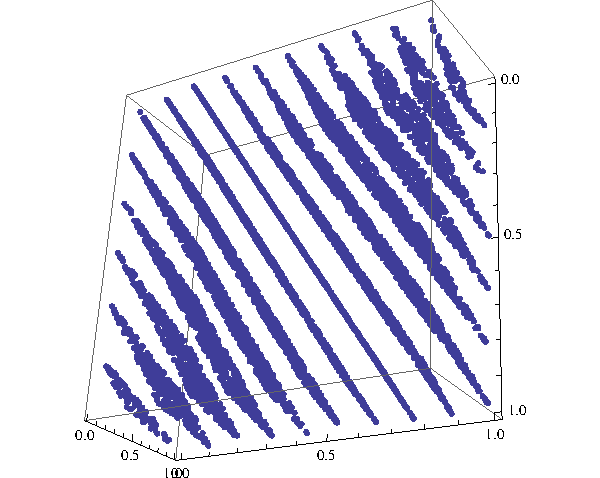
\includegraphics[scale=0.6]{randU.pdf}
  \caption{Performance of RandU in a three dimensional space. All the points lie on 15 planes in the space, making it a poor generator.}
  \label{fig:randU}
\end{figure}

\section{Methods}

\subsection{Random number generators}
\label{sec:rng}
\noindent In this report we test a few random number generators. Below is a list of those random generators with a small description of their construction and usage:
\begin{itemize}
  \item
    Mersenne Twister: A very popular random number generator invented in 1997 that uses matrix linear recurrence over binary fields to generate random numbers. This algorithm solves a lot of flaws earlier PRNG's had and also has a very large period of 2$^{19937}-1$, which is enough for most practical purposes. Next to this the algorithm is also very fast. Currently there is an even faster version available, SFMT, which is an improved variant of the original Mersenne Twister. Since we are interested in quality rather than speed, we will only use the original version in this report.
  \item
    rand: The standard random function in C/C++. This is a linear congruential generator as described in the previous section with $a$ = 1103515245, $b$ = 12345 and $m$ = $2^{32}$. It has the same shortcomings linear congruential generators always have (see the previous section) but nonetheless serves a basic purpose for small programmes (since the period is small).
  \item
    random: Has the same properties as rand with a slightly longer period.
  \item
    rand48: Another linear congruential generator, but this time performing arithmetic on 48 bits (instead of 32). The linear congruential generator has parameters $a$ = 5214903917, $b$ = 11, $m$ = $2^{48}$. One of the advantages is a large cycle period and better randomness in lower bits compared to rand.
  \item
    R250: A random number generator from the 80s using a shift register sequence with exclusive-or operatoins. It is very fast and has a very long period and it was a popular random number generator for a long time (until the discovery of Mersenne Twister). This PRNG is included in the GNU Scientific Library.
  \item
    RandU: See the previous section for a discussion on RandU. This PRNG is also included in the GNU Scientific library.
  \item 
    Quantis: Quantis is a random number generator using a quantum optics device to generate random numbers. Since the process is quantummechanical (hence probabilistic) in nature, this random generator is believed (and tested) to be truly random and hence it should pass all possible tests. Unfortunately we only have access to $10^6$ numbers generated with this device, which is not enough to run very accurate tests. 
\end{itemize}

\subsection{Kolmogorov-Smirnov test}
There are many tests for determining the quality of a RNG. We will use one that is not a direct test, but rather an indirect one, doing statistics on results generated with one of the RNG's above.\\
\noindent To this purpose we define a random walk on a two dimensional lattice by looking at the last and second last significant bits of a random number. If the last bit is zero, step to the left, if it is one, step to the right. If the second last bit is zero step up, otherwise step down. By starting on a 2D lattice with starting point (0,0) the endpoints can be determined after a number of steps on the lattice, $N_{\text{steps}}$. A PRNG can be tested by using it to generate the random numbers for the random walk and observing the end point of the random walk after $N_{\text{steps}}$. The endpoint lies (with an odd number of steps) always in one of the four quadrants in the 2D plane. By doing a number of random walks $N_{\text{walks}}$ the number of walks that end up in each quadrant can be counted. From these counts a $\chi^2$ value can be determined as follows:
\begin{equation}
\chi^2 = \sum_{i=0}^{N_{\text{quadrants}}-1} \frac{(O_{i} - E_{i})^2}{E_{i}}
\end{equation}
\noindent where $N_{\text{quadrants}} = 4$, $O_{i}$ is the observed number of walks with end points in quadrant $i$ and $E_{i} = \frac{N_{\text{walks}}}{4}$ is the expected number of walks with end points in quadrant $i$. A large $\chi^2$ value implies an overrepresentation for a certain quadrant.\\
\noindent By repeating this experiment a number of times $N_{\text{samples}}$ a series of $\chi^2$ are obtained. If the random number generator is truly random (or random 'enough') the $\chi^2$ values will follow a cumulative $\chi^2$ distribution defined by:
\begin{equation}
\label{eq:1}
\chi_{k}^{2}(x) = \frac{\gamma(k/2,x/2)}{\Gamma(k/2)}
\end{equation}
where $k$ is the number of degrees of freedom, in this case $k = 3$. Furthermore $\gamma$ is the lower incomplete gamma function and $\Gamma$ is the regular gamma function \cite{book}.\\
\noindent The Kolmogorov-Smirnov (or KS) is a test which gives a value, called the D-value, which describes how well the observed values, in this case the $\chi^2$ follow a certain distribution, in this case the $\chi^2$ distribution. The D-value for a Kolmogorov-Smirnov test is given by:
\begin{equation}
\text{D} = \text{max} \; \{ \frac{j}{n} - F(y_{j}),F(y_{j}) - \frac{j-1}{n}, j = 1,....,n \}
\end{equation}
\noindent where $n = N_{\text{samples}}$ is the number of observed values, $F(y_{i})$ is the function evaluation in the observed value $y_{i}$, where $y_{i}$, $i = 0,...,n$ is an ordered list of the observed values. The obtained D-value is itself distributed according to a certain complicated distribution function \cite{kolmogorov}. By consulting a table for the distribution the D-values, see \cite{table} and choosing a confidence interval the calculated D-value can be accepted or rejected. If the D-value is accepted, it means that it lies within the range of expected D-values and so our assumption that the RNG generating the random walks is truly random, is accepted. Otherwise, the calculated D-value is unlikely to be found and we reject our assumption that the RNG is truly random. Note that the D-value is a function of $N_{\text{samples}}$, scaling with the reprocical of the square root of $N_{\text{samples}}$.

\subsection{Statistical variables}
Next to the KS-test mentioned in the previous section, we will also do some further analysis on the statistics of the random walks. Specifically, we will calculate the average and the standard deviation (defined in the standard way) of the squared 2-norm of the end points of the random walks. We first compute the average norm within one test (hence computing the average over $N_{\text{walks}}$ random walks) and then after taking $N_{\text{samples}}$ we take the average over all samples and calculate a corresponding standard deviation. For a 2D lattice the average length of the path should be close to $l \sqrt{N_{\text{steps}}}$ where $l = \sqrt{2}$ is the step size, since we perform up/down and left/right in one step \cite{book2}.\\
\noindent We also calculate a $\chi^2$ value over the whole test, using equation \ref{eq:1} but now counting all the end points over all the samples, and hence an expected value $E_{i} = \frac{N_{\text{samples}}*N_{\text{walks}}}{4}$. A very large value for the resulting $\chi^2$ might also indicate that something is wrong, since it indicates a preference for a certain quadrant.

\subsection{Diehard package}
The Diehard package is a package of statistical tests in which all tests are designed to test random number generators on their randomness. The package we used comes from source \cite{diehard} and contains fifteen tests, among which the famous birthday test. For all RNG's described above $10^7$ random numbers were generated and used as input for the tests.

\section{Results}
\subsection{KS-test results}
We use the random number generations defined in section \ref{sec:rng} and perform a KS-test on all of them. We choose the number of steps $N_{\text{steps}} = 1001$ and $10001$, the number of $N_{\text{walks}} = 1000$ and the number of $N_{\text{samples}} = 1000$. For every RNG we compute a D-value, a $\chi^2$ over the total data and an average path length with an error with a confidence level of 1$\%$. The following three tables, one for each $N_{\text{steps}}$, show these quantities for all the RNG's defined in section \ref{sec:rng} for the same seed value 9287348. The last column of the tables states whether a RNG should be accepted or rejected as a true random number generator, based on the calculated D-value and a confidence level of $1\%$, given by the table from \cite{table}:

\begin{center}
\begin{table}[H]
\begin{tabular}{l *{4}{c} r}
\hline
\multicolumn{6}{c}{$N_{\text{steps}}$ = 1001, critical D-value 0.048000}\\
\hline
PRNG & D-value & $\chi^2_{\text{total}}$ & Average path length & Expected path length & Accept/Reject\\
\hline
rand &  0.063723 & 160.293488 & 2002.2 $\pm$ 5.1 & 2002 & reject\\
random &  0.063723 & 160.293488 & 2002.2 $\pm$ 5.1 & 2002 & reject\\
rand48* & 0.080730 & 0.026408 & 2001.1 $\pm$ 2.6 & 2002 & reject\\
Mersenne Twister & 0.019102 & 2.288984 & 2001.0 $\pm$ 5.1 &  2002 & accept\\
R250* & 0.253539 & 1898.290649 & 2001.2 $\pm$ 5.1 & 2002 & reject\\
RandU* & 1.00000 & 10$^6$ & 10$^6$ $\pm$ 0.1 & 2002 & reject\\
\hline
\end{tabular}
\newline
\begin{tabular}{l *{4}{c} r}
\hline
\multicolumn{6}{c}{$N_{\text{steps}}$ = 10001, critical D-value 0.048000}\\
\hline
PRNG & D-value & $\chi^2_{\text{total}}$ & Average path length & Expected path length & Accept/Reject\\
\hline
rand &  0.018427 & 6.822216 & 20009 $\pm$ 53 & 20002 & accept\\
random & 0.018427 & 6.822216 & 20009 $\pm$ 53 & 20002 & accept\\
rand48* & 0.533604 & 0.024024 & 20333 $\pm$ 15 & 20002 & reject\\
Mersenne Twister & 0.031996 & 4.686152 & 20003 $\pm$ 51 & 20002 & accept\\
R250* & 0.278678 & 1853.408325 & 21314 $\pm$ 3278 & 20002 & reject\\
RandU* & 1.00000 & 10$^6$ & 10$^8$ $\pm$ 107 & 20002 & reject\\
\hline
\end{tabular}
\caption[width=5.0cm]{Results for the KS-test for different random number generators, as well as some statistical quantities. The last column gives whether the PRNG is accepted or rejected as a true random number generator based on the $D$-value and a confidence level of $1\%$.\\
*The bits considered here are not the last and second to last bit, but the 3rd and 4th to last bit. For an explanation see text.}
\end{table}

\end{center}

\noindent In the first table shown above 5 out of 6 tests fail, while in the second table only 3 out of 6 tests fail, noting that rand and random give the same results. The difference in the number of failed tests is due to the increased $N_{\text{steps}}$ in the second table, which makes the test much more accurate. Another interesting fact is that it was not possible for rand48, R250 and RandU to extract any sensible data from the first two bits, hence then next two bits are used in the test. In the case of RandU this is because of the last bit being always odd or even and even for other bits it always produces the same paths, leading to a very large average path length compared to the expected value. For rand48 however, the numbers generated are too uniform, which can be seen by a very low $\chi^2_{total}$. For R250 the numbers generated are not uniform enough. This is an important result. For rand48 and R250 this effect is still present in the more significant bits, but it diminishes for increasing significance of the bits. For rand48 this uniformness leads to low values for the computed $\chi^2$ and hence the test with a real $\chi^2$ distribution fails (which allows some high $\chi^2$ values). For R250 it is the other way around, the computed $\chi^2$ values are much higher than would be expected from the distribution. The figures shown below gives the $\chi^2$ distribution together with the data for rand (left) and rand48 (right). The dotted line gives the difference between the theoretical $\chi^2$ distribution and the observed values. The abundance of low $\chi^2$ values when using rand48 is easily seen in this way, while the data follows the curve nicely for rand.
\newline
\noindent From the tables we can conclude that when comparing all the PRNG's that we have tested, the Mersenne Twister is the one with the most accurate results because, like rand and random, it passes the test, but it also gives a small $\chi^2_{total}$, which means that when summing up all the paths and looking in which quadrant the endpoint lies, it still gives a good distribution. It is remarkable that rand and random perform so well, because they are generally believed to be poor generators. On the other hand, rand48 is believed to be reasonably good, while these tests show that this is indeed not the case. However if one is looking for a very uniform random number generator, rand48 might serve this purpose well.

\begin{figure}[H]
  \centering
  \subfloat{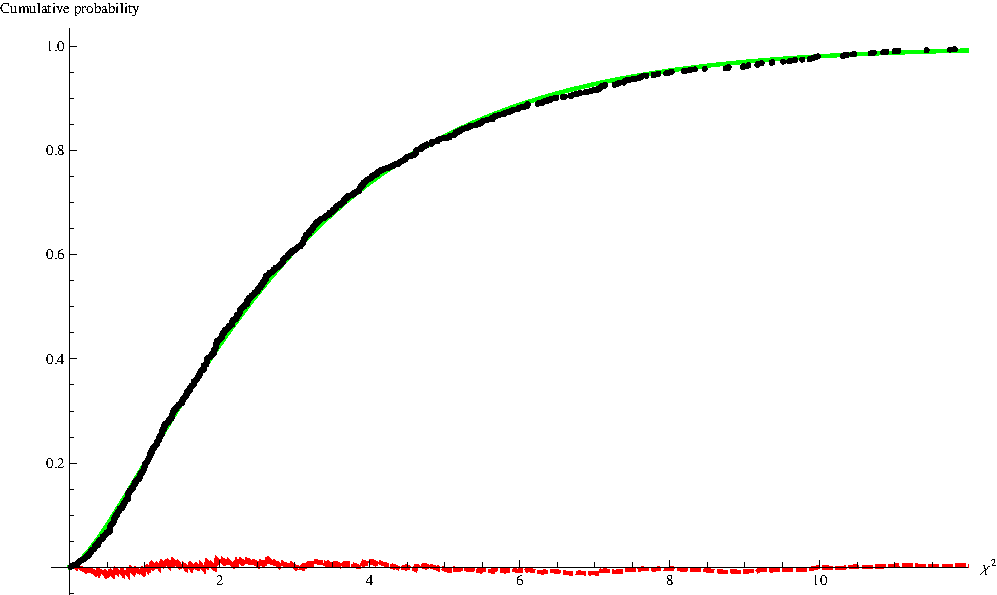
\includegraphics[width=0.5\textwidth]{rand_test.pdf}}    
  \subfloat{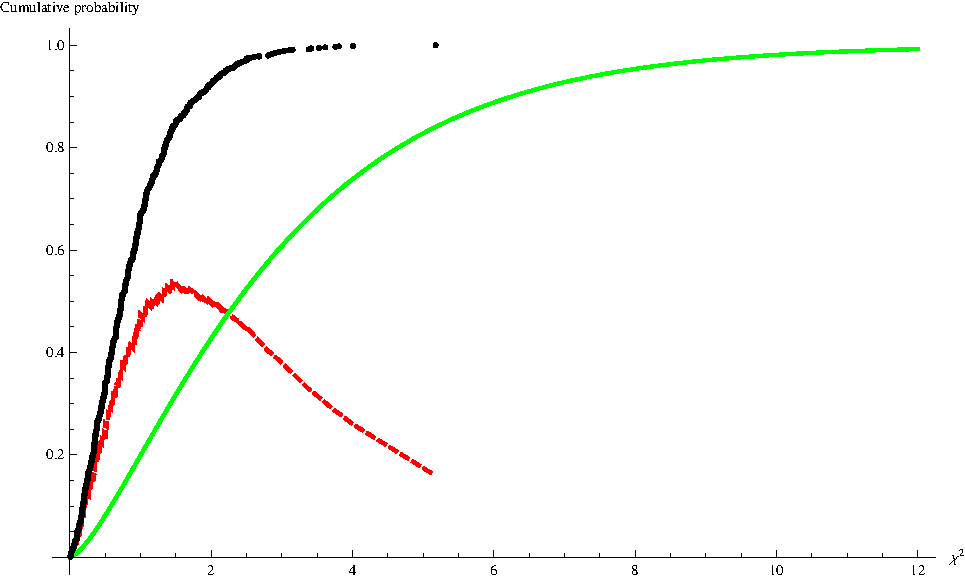
\includegraphics[width=0.5\textwidth]{rand48_test.pdf}}
  \caption{The $\chi^2$ distribution (green line) together with the computed $\chi^2$ values (black dots) and the difference between them, evaluated pointwise (red dots). The left figure shows data from rand, the right from rand48.}
  \label{fig:compare}
\end{figure}

\begin{figure}[H]
  \centering
  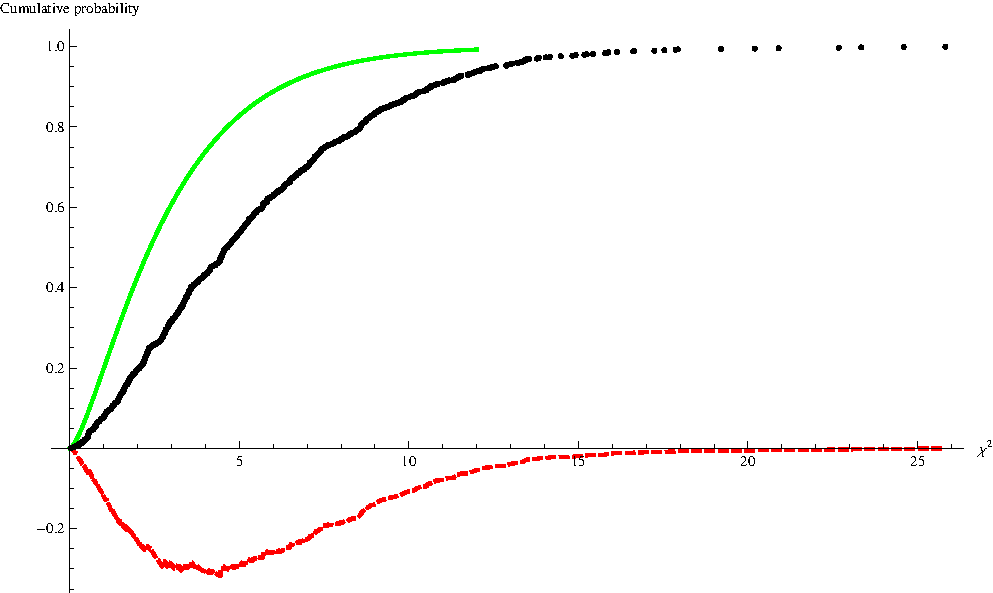
\includegraphics[scale=0.5]{r250_test.pdf}
  \caption{The $\chi^2$ distribution (green line) together with the computed $\chi^2$ values (black dots) and the difference between them, evaluated pointwise (red dots). For the $\chi^2$ values the R250 RNG is used.}
  \label{fig:r250}
\end{figure}

\noindent Figure \ref{fig:r250} shown below gives this same data for the R250 random number generator. In this case, opposite to the situation in the figure above, the $\chi^2$ values from the data are much larger than the distribution prescribes and hence this random generator also performs very poorly.

\noindent Apart from the PRNG's mentioned in the table, also a KS-test was performed with numbers available from Quantis, a physical random number generator using an optical device to generate its random numbers \cite{quantis}. Since this is a quantum process, the random numbers generated with this device should be truly random and hence pass all possible tests. Since we only have access to $10^6$ numbers generated with this device, we did a KS-test with $N_{\text{steps}}$ = 10001, $N_{\text{walks}}$ = 10 and $N_{\text{samples}}$ = 10, giving a D-value of 0.191978, with a critical D-value of 0.4566 and hence, as expected, Quantis passes the KS-test.

\subsection{Diehard tests}
Next to the Kolmorgorov-Smirnov on a $\chi^2$ distribution for random walks, we also generated 10$^7$ random numbers from the various RNG's defined before and run them through a package of statistical tests called the Diehard tests available at \cite{diehard}. This package contains the famous birthday tests, among 14 other tests. Due to the small amount of random numbers available from the Quantis generator, we were only able to perform the birthday test with this random number generator. In table \ref{tab:diehard} shown below the test results are given:

\begin{center}
\begin{table}[H]
  \centering
\begin{tabular}{l c r}
\hline
PRNG & Passed birthday test? & Test score (out of 15)\\
\hline
rand &  no & 1\\
random &  no & 1\\
rand48 & yes & 1\\
Mersenne Twister & yes & 11\\
R250 & yes & 9\\
RandU & no & 0\\
Quantis & yes & not available \\
\hline
\end{tabular}
\caption[width=5.0cm]{Test results for the various RNG's, the test score includes the birthday test.}
\label{tab:diehard}
\end{table}
\end{center}

\noindent The results from the table show that the Mersenne Twister has the best score, followed by R250. It is remarkable that R250 scores so well, given the bad results for the KS-test. Something else which is remarkable is that rand (and also random) perform very bad in the tests, while they performed very well in the KS-test. Both RandU and rand48 performed badly, which is expected also from the KS-test.

\section{Discussion}

\noindent The results above show some interesting results, namely there is a difference between the outcome of the Diehard package and between the KS-test. Though there are differences, both methods show that the Mersenne Twister is a reliable random number generator which produces the best results among the different RNG's tested in this report. The behavior found with the KS-test in rand48 and R250 is remarkable, since they are both considered as fairly good random number generators. Quantis passes the tests that are performed on it, but as said before, we could do only do a limited number of tests.\\
\newline
\noindent The discrepancy between the results for the KS-test and the Diehard package might indicate that the testing method used for the KS-test, the random walks, might be a bit too simple and not take into account other aspects of random number generators, which are tested in the Diehard package. It is however still remarkable that especially in the least significant bits most of the generators perform poorly. Also the results obtained in the figures \ref{fig:compare} and \ref{fig:r250} leave little doubt that the results for the D-value cannot be simply related to a statistical exception (i.e. one $\chi^2$ in the wrong place) but instead  it seems to indicate that something goes structurally wrong in the algorithm behind the random number generator. Another remarkable thing is that the standard C/C++ random function, rand, passes the KS-test but fails in the Diehard test package. This might also indicate that the KS-test focuses on a single aspect of random number generation (the randomness of least significant bits) but fails to grasp on other aspects which are just as important (for instance in looking at the randomness of the total number that is generated).\\
\newline
\noindent After doing this project I would definitely, based on the results, use the Mersenne Twister whenever possible (or the faster version, which I have not tested in this report). My expectation in the beginning of this project was that I most likely would not find any significant poor results for any of the random number generators, except maybe RandU. However, it turned out flaws in the random number generated can be discovered to some extent with the random walk method and the KS-test on this. I did all the tests multiple times, with different seeds and different sample/test/step sizes to check for consistency. It seems that one actually needs bigger step sizes and samples (in the order of millions) to get a much more reliable test statistic. This can already be seen by comparing the different step sizes in the previous section, more random number generators pass for larger step size.

\subsection{About the code}
All the work is done in the program rng\_test.c. It calculates a series of $\chi^2_{j}$ for each sample $j$ and outputs this to a file together with the value $\frac{j+1}{N_{\text{samples}}}$ which assumes the $\chi^2_{j}$ follow a real $\chi^2$ distribution. Also, it computes the D-value, a mean squared norm and a standard deviation of the mean squared norm and outputs these last two to a file. Also it computes a $\chi^2$ value over all the samples. It takes about 2 minutes to run 10001 steps, 1000 walks and 1000 samples. The sorting algorithm which is used to sort the array of $\chi^2$ values per sample is insert sort, which is easy to implement and has reasonably good results for arrays which are not too long, in this case the array has 1000 elements. Mathematica is used to produce the figures in the report with a few basic Mathematica routines.

\begin{thebibliography}{15}
\bibitem{quantis}
  http://www.idquantique.com/true-random-number-generator/products-overview.html 
\bibitem{diehard}
  http://www.stat.fsu.edu/pub/diehard/
\bibitem{lavalamp}
  http://www.lavarnd.org/
\bibitem{decay}
  http://www.fourmilab.ch/hotbits/
\bibitem{human}
  http://www.wisdom.weizmann.ac.il/$\sim$neko/MAE-offline.html
\bibitem{lcg}
  http://en.wikipedia.org/wiki/Linear\_congruential\_generator
\bibitem{marsaglia}
  Eichenauer, J., Grothe, H, Lehn, J., 1988, Metrika, Vol. 35, \#1, 241-250
\bibitem{book}
  Ross, S.M., \emph{Simulation}, 2006, Academic Press
\bibitem{kolmogorov}
  Marsaglia, G., Tsang, W. W., Wang, J., 2003, Journal of Statistical Software, 8 (18), 1–4
\bibitem{table}
  http://www.york.ac.uk/depts/maths/tables/
\bibitem{book2}
  Newman, M.E.J., Barkema, G.T., \emph{Monte Carlo methods in Statistical Physics}, 1999, Oxford University Press
\end{thebibliography}

\end{document}